\documentclass[a1paper]{article}

% --- Page and packages ---
\usepackage[a1paper,margin=30mm]{geometry}
\usepackage{tikz}
\usetikzlibrary{calc,arrows.meta,positioning}
\usepackage{graphicx}
\usepackage{booktabs}
\usepackage{mwe}     % dummy images: example-image-a/b/c/...
\usepackage{helvet}
\usepackage[most]{tcolorbox}
\usepackage{caption}
\usepackage{varwidth}
\usepackage{enumitem}
\usepackage{xcolor}
\usepackage{pagecolor}
\usetikzlibrary{backgrounds}


\renewcommand{\familydefault}{\sfdefault}
\pagestyle{empty}

% --- Styles and sizes ---
\tikzset{
  img/.style = {draw, rounded corners=6pt, very thick, align=center, inner sep=0pt},
  tbl/.style = {draw, rounded corners=6pt, very thick, align=center, inner sep=6pt},
  arrow/.style = {->, >=Latex, very thick}
}

% Portrait / landscape / small image sizes
\newcommand{\wPortrait}{0.07\paperheight}
\newcommand{\hPortrait}{0.09\paperheight}
\newcommand{\wLandscape}{0.24\paperwidth}
\newcommand{\hLandscape}{0.16\paperheight}
\newcommand{\wSmall}{0.10\paperwidth}
\newcommand{\hSmall}{0.10\paperheight}

\definecolor{table_header}{RGB}{2, 30, 82}
\definecolor{title_color}{RGB}{1, 25, 69}
\definecolor{title_frame_color}{RGB}{0, 0, 0}
\definecolor{variable_color}{RGB}{152, 31, 31}
\definecolor{first_level_color}{RGB}{179, 85, 65}
\definecolor{second_level_color}{RGB}{128, 128, 128}

\definecolor{orange2}{HTML}{f7972f}



\newtcolorbox{mybox}[1]{
  varwidth boxed title,
  enhanced,
  attach boxed title to top center={yshift=-3mm,yshifttext=-1mm},
  boxed title style={size=small, coltitle=title_color, colback=title_color, colframe=title_frame_color},
  center title,
  colback=blue!1!white,
  title={#1},
  top=1pt, bottom=-1pt, left=3pt, right=3pt,
  width=0.95\columnwidth
}

\newtcolorbox{first_level}[1]{varwidth boxed title, enhanced,attach boxed title to top center={yshift=-3mm,yshifttext=-1mm},
boxed title style={size=small, coltitle=black, colback=title_color, colframe=title_frame_color}, 
center title, colback=blue!1!white, title={#1}, top=5pt, bottom=0pt, left=3pt, right=3pt, width=0.95\columnwidth}

\newtcolorbox{second_level}{colback=gray!1!white, colframe=second_level_color, top=1pt, bottom=0pt, left=3pt, right=3pt}


\definecolor{background}{HTML}{ebf0f7}

\begin{document}

\pagecolor{background}


% -------- Title --------
\begin{center}
  \vspace*{2mm}
  {\fontsize{56}{56}\selectfont {\color{table_header}\textbf{Munich\_Z@GermEval Shared Task 2025:When Prompting Is Not Enough: The Limits of Large Language Models in GermEval’s 2025 Harmful Content Detection Task}}}
\end{center}



% -------- Canvas (absolute placement in 0..1 × 0..1) --------
\begin{tikzpicture}[remember picture,overlay, x=\paperwidth, y=\paperheight]
\begin{scope}[shift={(current page.south west)}]

\node[draw=none, rounded corners=6pt, align=center, anchor=east] 
at (0.95, 0.95) {

\begin{minipage}{0.9\paperwidth}
    \centering
   {{\fontsize{56}{56}\selectfont \color{white} \textbf{Munich\_Z@GermEval Shared Task 2025:When Prompting Is Not Enough: The Limits of Large Language Models in GermEval’s 2025 Harmful Content Detection Task}
   }}
\end{minipage}
};



\node[draw=none, rounded corners=6pt, align=center, anchor=east] 
at (0.4, 0.90) {{\fontsize{32}{32}\selectfont \color{white} Florian Ludwig}};
\node[draw=none, rounded corners=6pt, align=center, anchor=east] 
at (0.7, 0.90) {{\fontsize{32}{32}\selectfont \color{white} Dr. Stefan Altmann}};

\node[draw=none, rounded corners=6pt, align=center, anchor=east] 
at (0.43, 0.885) {{\fontsize{24}{24}\selectfont \color{white} florian.ludwig@zitis.bund.de}};
\node[draw=none, rounded corners=6pt, align=center, anchor=east] 
at (0.71, 0.885) {{\fontsize{24}{24}\selectfont \color{white} stefan.altmann@zitis.bund.de}};


% ======================= First Image ===================================================

% Title scope
\begin{scope}[on background layer]
    \fill[table_header](0\paperwidth,0.86\paperheight) 
                 rectangle (1\paperwidth, 1\paperheight);
\end{scope}


% Motivation Header
\begin{scope}[on background layer]
    \fill[table_header, draw=table_header, line width=5pt](0.015\paperwidth, 0.815\paperheight) 
                 rectangle (0.5\paperwidth, 0.85\paperheight);
\end{scope}

% Motivation
\begin{scope}[on background layer]
    \fill[white, draw=table_header, line width=5pt, ](0.015\paperwidth,0.475\paperheight) 
                 rectangle (0.5\paperwidth, 0.815\paperheight);
\end{scope}


% Results and Analyzis Header
\begin{scope}[on background layer]
    \fill[table_header, draw=table_header, line width=5pt](0.53\paperwidth, 0.815\paperheight) 
                 rectangle (0.985\paperwidth, 0.85\paperheight);
\end{scope}

% Results and Analyzis
\begin{scope}[on background layer]
    \fill[white, draw=table_header, line width=5pt, ](0.53\paperwidth,0.475\paperheight) 
                 rectangle (0.985\paperwidth, 0.815\paperheight);
\end{scope}


% Prompting Strategies Header
\begin{scope}[on background layer]
    \fill[table_header, draw=table_header, line width=5pt](0.015\paperwidth, 0.445\paperheight) 
                 rectangle (0.5\paperwidth, 0.41\paperheight);
\end{scope}

% Prompting Strategies
\begin{scope}[on background layer]
    \fill[white, draw=table_header, line width=5pt](0.015\paperwidth,0.41\paperheight)   
                 rectangle (0.5\paperwidth, 0.015\paperheight);
\end{scope}


% Examples Header
\begin{scope}[on background layer]
    \fill[table_header, draw=table_header, line width=5pt](0.53\paperwidth, 0.26\paperheight) 
                 rectangle (0.985\paperwidth, 0.225\paperheight);
\end{scope}


% Exampels
\begin{scope}[on background layer]
    \fill[white, draw=table_header, line width=5pt](0.53\paperwidth,0.225\paperheight) 
                 rectangle (0.985\paperwidth, 0.015\paperheight);
\end{scope}



\node[draw=table_header, align=center, anchor=east] 
at (0.325, 0.8325) {{\fontsize{40}{40}\selectfont \color{white} \textbf{Motivation}}};

\node[img, rounded corners=0pt, draw=table_header, line width=4pt, inner sep=0pt, minimum width=\wPortrait, minimum height=\hPortrait] (img1) at (0.18, 0.76)
{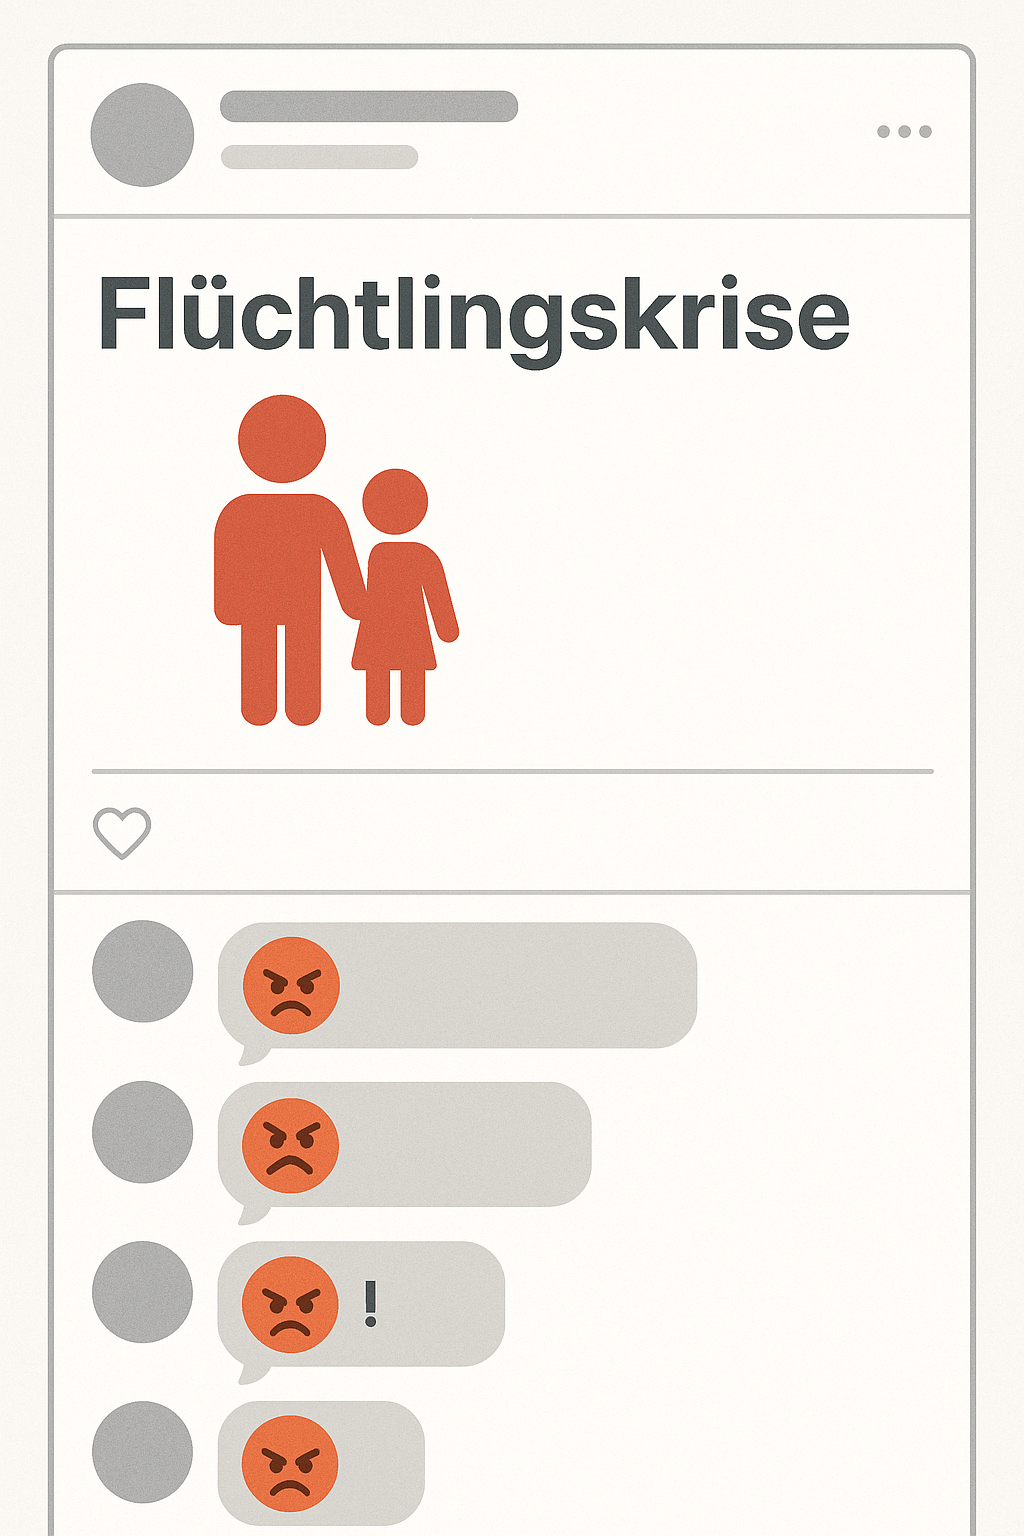
\includegraphics[width=\wPortrait,height=\hPortrait]{imgs/refugees.png}};

\node[img, rounded corners=0pt, draw=table_header, line width=4pt, inner sep=0pt, minimum width=\wPortrait, minimum height=\hPortrait] (img2) at (0.38, 0.76)
{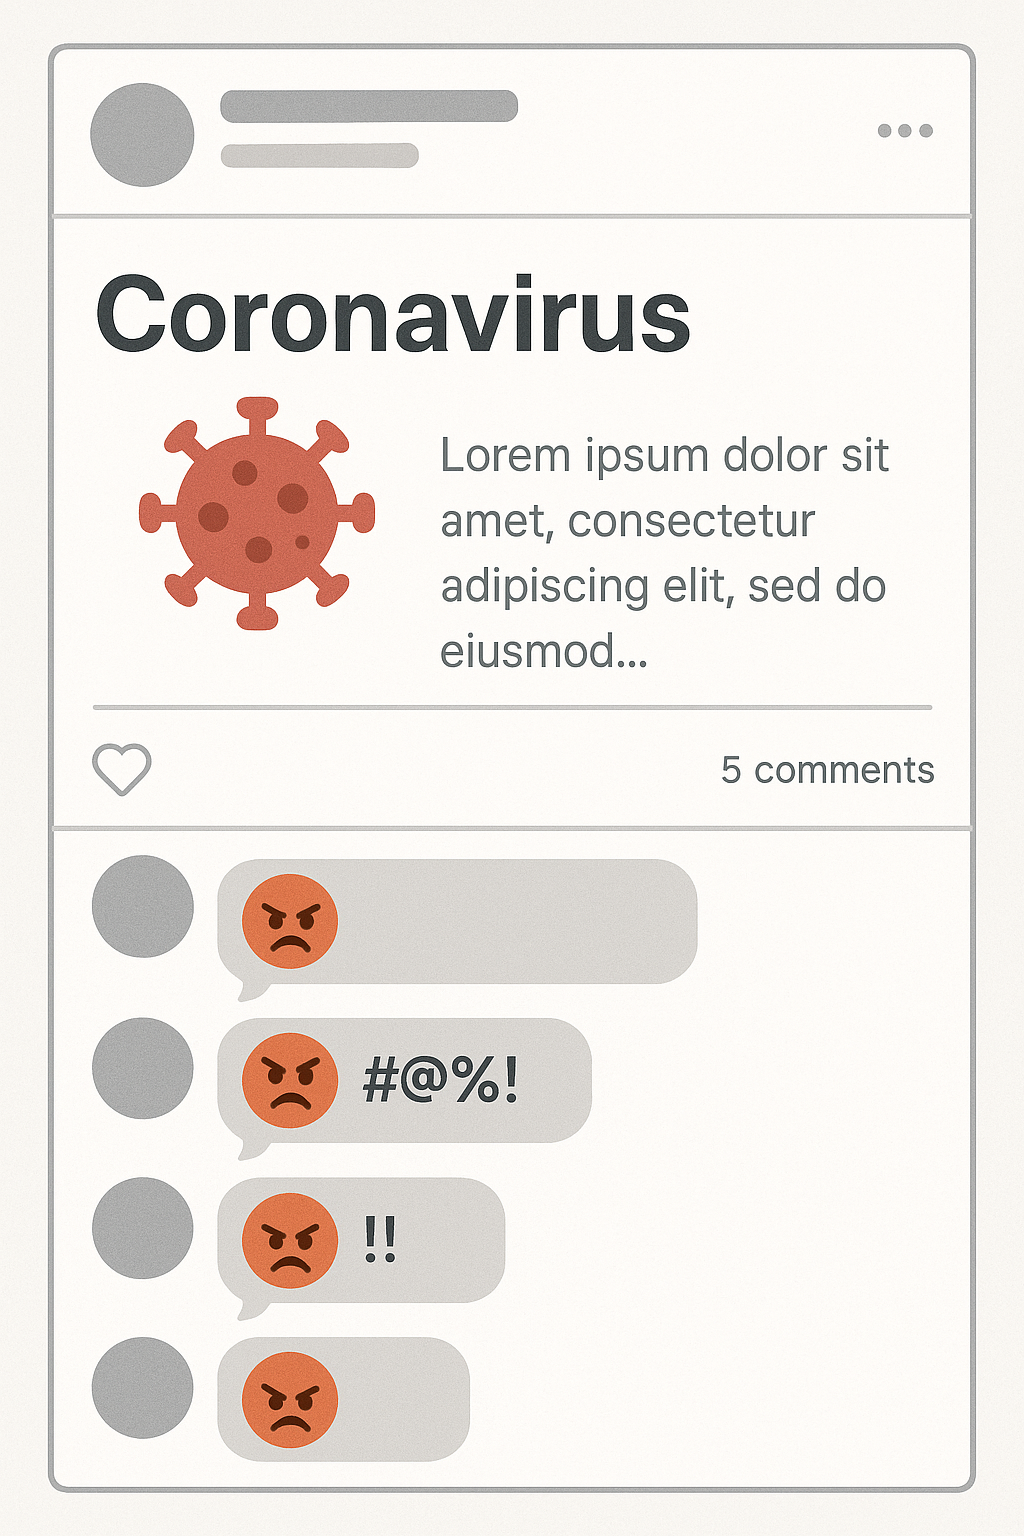
\includegraphics[width=\wPortrait,height=\hPortrait]{imgs/corona.png}};

\node[img, rounded corners=0pt, draw=table_header, line width=4pt, inner sep=0pt, minimum width=\wPortrait, minimum height=\hPortrait] (img3) at (0.38, 0.65)
{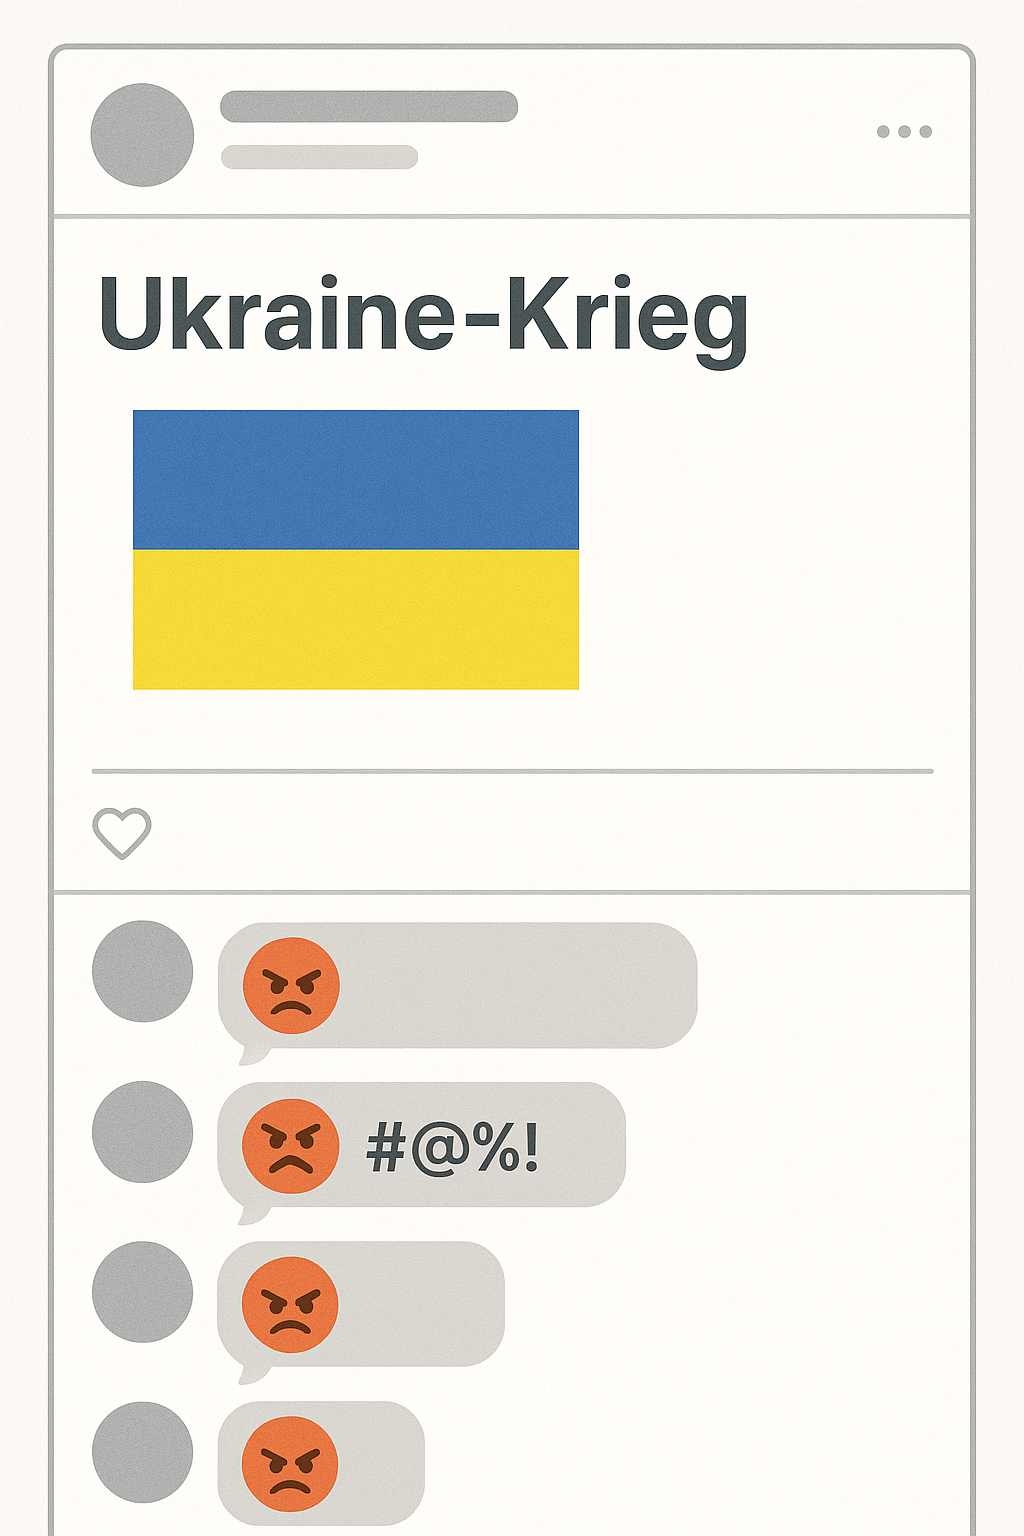
\includegraphics[width=\wPortrait,height=\hPortrait]{imgs/ukraine.png}};

\node[img, rounded corners=0pt, draw=table_header, line width=4pt, inner sep=0pt, minimum width=\wPortrait, minimum height=\hPortrait] (img4) at (0.18, 0.65)
{
\includegraphics[width=\wPortrait,height=\hPortrait]{imgs/israel.png}};

% Arrows across the top
\draw[arrow, table_header, line width=4pt] (img1.east) -- ($(img1.east)!1.0!(img2.west)$);
\draw[arrow, table_header, line width=4pt] (img2.south) -- ($(img2.south)!1.0!(img3.north)$);
\draw[arrow, table_header, line width=4pt] (img3.west) -- ($(img3.west)!1.0!(img4.east)$);
\draw[arrow, line width=4pt, table_header] (img4.west) -- ++(-2cm,0);
\draw[arrow, line width=4pt, table_header] ($(img1.west)+(-2cm,0)$) -- (img1.west);

% Dotted points
\node[draw=table_header, rounded corners=6pt, align=center, anchor=east] 
  at ($(img1.west)+(-2.5cm,0)$) {{\fontsize{70}{70}\selectfont \color{table_header} ...}};

\node[draw=table_header, rounded corners=6pt, align=center, anchor=east] 
  at ($(img4.west)+(-2.5cm,0)$) {{\fontsize{70}{70}\selectfont \color{table_header} ...}};


\node[draw=none, rounded corners=6pt, align=center, anchor=east] 
at (0.4, 0.535) {
\begin{minipage}{0.325\paperwidth}
   {{\fontsize{27.5}{27.5}\selectfont \color{table_header} 
   
   \begin{itemize}[itemsep=0.5cm]
       \item Hateful language is highly dynamic and follows trends.
       \item Machine Learning models need to be quickly adapted to the language.
       \item Zero-Shot and Few-Shot prompting of Large Language Models could be suitable for these problems.
   \end{itemize}
   }}
\end{minipage}
};
  

% ======================= Approaches ===================================================


\node[draw=none, rounded corners=6pt, align=center, anchor=east] 
at (0.37, 0.425) {{\fontsize{40}{40}\selectfont \color{white} \textbf{Prompting Strategies}}};

\node[draw=none, inner sep=0pt] (fig1) at (0.14,0.335) {
  \begin{minipage}{0.22\paperwidth}
        {\fontsize{20}{20}\selectfont
            \begin{mybox}{\textbf{Task Description}}
                
                \vspace{0.5cm}
                
                \textcolor{title_frame_color}{\textbf{Subversive:}} 
                                
                \textcolor{black}{\it{Subversive posts express the aim of overthrowing the government [...]}}
                        
                \vspace{0.5cm}
            
                \textcolor{title_frame_color}{\textbf{Agitational:}} 
                            
                \textcolor{black}{\it{Posts in the "Agitational" category aim to incite others aggressively [...]}}
                    
                \vspace{1cm}
                            
                \textcolor{title_frame_color}{\textbf{Instruction: }} 
                            
                \textit{Classify the following post into exactly one of the above categories.}
                    
                \vspace{1cm}
                    
                \textcolor{title_frame_color}{\textbf{Post: }} 
                            
                \textbf{\textcolor{variable_color}{\textbf{Post to classify}}}
        
            \end{mybox}
        }
  \end{minipage}
};


\node[draw=none, inner sep=0pt] (fig1) at (0.36,0.335) {
  \begin{minipage}{0.22\paperwidth}
        {\fontsize{20}{20}\selectfont
            \begin{mybox}{\textbf{Chain of Thought}}
            
            \vspace{0.5cm}
            
            \textcolor{title_frame_color}{\textbf{Subversive:}} 
                            
            \textcolor{black}{\it{Subversive posts express the aim of overthrowing the government [...]}}        

            [...]
            \vspace{0.7cm}

            \textcolor{title_frame_color}{\textbf{Instruction: }} 
                        
            \textit{Classify the following post into exactly one of the above categories. Think step by step how you can solve this task. Think about which characteristics the individual classes [...]}
                
            \vspace{1cm}
                
            \textcolor{title_frame_color}{\textbf{Post: }} 
                        
            \textbf{\textcolor{variable_color}{\textbf{Post to classify}}}
        \end{mybox}
    }
  \end{minipage}
};


\node[draw=none, inner sep=0pt] (fig1) at (0.14,0.14) {
  \begin{minipage}{0.22\paperwidth}
        {\fontsize{20}{20}\selectfont
        \begin{first_level}{\textbf{In-Context Learning}}
            \vspace{0.15cm}
            \begin{second_level}
        
                \smallskip
        
                \textcolor{title_frame_color}{\textbf{Subversive:}} 
                        
                \textcolor{black}{\it{Subversive posts express the aim of overthrowing the government ...}}
                
                \vspace{0.5cm}
        
                [...]
        
                \vspace{1cm}
                
                \textcolor{title_frame_color}{\textbf{Instruction: }} 
                
                \textit{Classify the following post into exactly one of the above categories.}
        
                \vspace{1cm}
        
                \textcolor{title_frame_color}{\textbf{Post: }} 
                
                \textbf{\textcolor{variable_color}{\textbf{Example 1}}}
        
            \end{second_level}
            \vspace{0.5cm}
            \hspace{2.5 cm} \textbf{\textcolor{title_color}{[Example Answer 1]}}
            \vspace{0.5cm}
            \begin{second_level}
        
                \textcolor{title_frame_color}{\textbf{Post: }} 
                
                \textbf{\textcolor{variable_color}{\textbf{Example 2}}}
            
            \end{second_level}
            \vspace{0.5cm}
            \hspace{2.5cm} \textbf{\textcolor{title_color}{[Example Answer 2]}}
            
            \vspace{1cm}
            
            \hspace{5cm} {\color{table_header}[...]}
        
            \begin{second_level}
        
                \textcolor{title_frame_color}{\textbf{Post: }} 
                
                \textbf{\textcolor{variable_color}{\textbf{Post to classify}}}
            
            \end{second_level}
    
        \end{first_level}
    }
  \end{minipage}
};






\node[draw=none, inner sep=0pt] (fig1) at (0.36,0.14) {
  \begin{minipage}{0.22\paperwidth}
        {\fontsize{20}{20}\selectfont
            \begin{first_level}{\textbf{Task Decomposition}}
                \vspace{0.15cm}
                \begin{second_level}
                    
                    \smallskip
                                            
                    \textcolor{black}{\textit{Does the following post contain negative attitudes towards state institutions [...] ?}}
                            
                    \vspace{1cm}
                            
                    \textcolor{title_frame_color}{\textbf{Post: }} 
                                    
                    \textbf{\textcolor{variable_color}{\textbf{Post to classify}}}
                                    
                    \vspace{0.25cm}
                    
                \end{second_level}
                \vspace{0.7cm}
                \hspace{2.5cm} \textbf{\textcolor{title_color}{[Model Answer]}}
                \vspace{0.7cm}
                \begin{second_level}
                            
                    \textcolor{black}{\textit{Does the post call for violence against state actors? This includes [...]}}        
                    \end{second_level}
                    \vspace{0.7cm}
                    \hspace{2.5cm} \textbf{\textcolor{title_color}{[Model Answer]}}  
                    \vspace{0.7cm}
                
                \begin{second_level}
                            
                    \textcolor{black}{\textit{Does this post incite other anti-state but non-violent acts or does it spread propaganda or anti-constitutional symbols? [...]}}        
                \end{second_level}
                \vspace{0.7cm}
                \hspace{2.5cm} \textbf{\textcolor{title_color}{[Model Answer]}}  
                \vspace{0.7cm}
            \end{first_level}
    }
  \end{minipage}
};


% ============================= Results ==========================

\node[draw=none, rounded corners=6pt, align=center, anchor=east] 
at (0.885, 0.832) {{\fontsize{40}{40}\selectfont \color{white} \textbf{Results and Analyzis}}};


\node[img, rounded corners=0pt, draw=none] (img5) at (0.755, 0.71)
{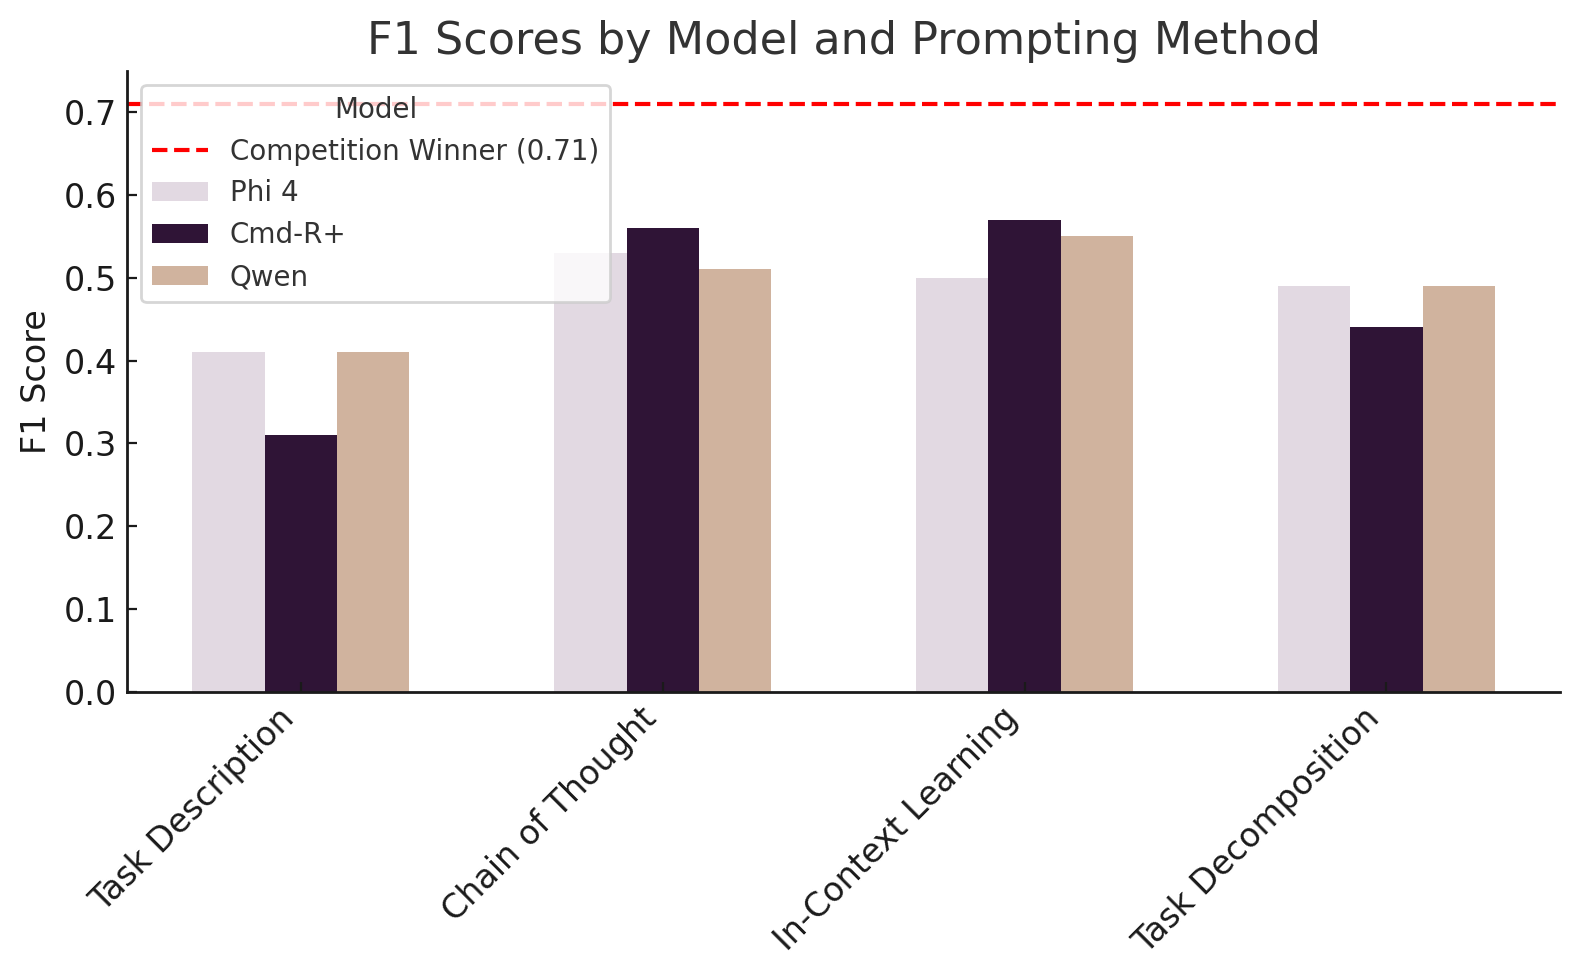
\includegraphics[width=0.42\paperwidth]{imgs/results.png}};



\node[draw=none, rounded corners=6pt, align=center, anchor=east] 
at (0.91, 0.55) {
\begin{minipage}{0.325\paperwidth}
   {{\fontsize{27.5}{27.5}\selectfont \color{table_header} 
   
   \begin{itemize}[itemsep=0.5cm]
       \item Language model prompting achieves worse results than other approaches.
       \item Most errors happen in the \textit{Subversive} class.
       \item Errors mainly arise from misunderstood or inaccurate class definitions and or incorrect data annotation.
   \end{itemize}
   }}
\end{minipage}
};



\node[draw=none, rounded corners=6pt, align=center, anchor=east] 
at (0.89, 0.24) {{\fontsize{40}{40}\selectfont \color{white} \textbf{Exemplary Error Cases}}};

\node[img, rounded corners=0pt, draw=none] (img6) at (0.76, 0.12)
{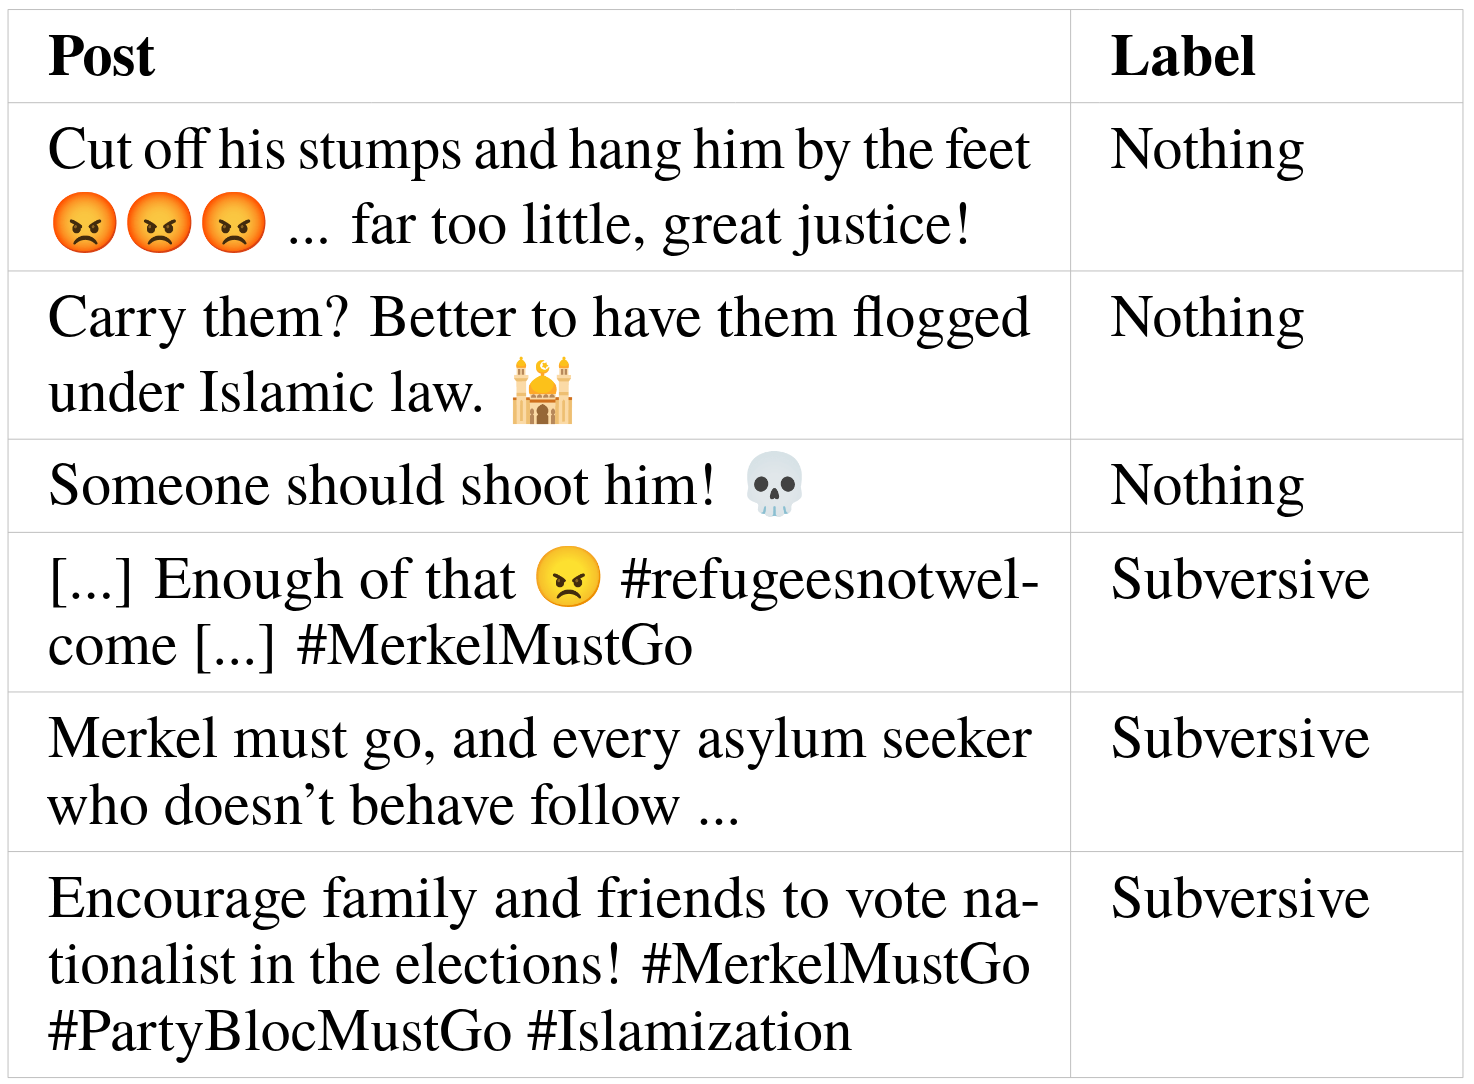
\includegraphics[width=0.38\paperwidth]{imgs/table.png}};




\end{scope}
\end{tikzpicture}

\end{document}
